\documentclass[a4paper, 11pt]{article}
\usepackage[left=2cm,top=3cm,text ={17cm,24cm}]{geometry}
\usepackage[czech]{babel}
\usepackage[utf8]{inputenc}
\usepackage{times}
\usepackage{amssymb}
\usepackage{amsmath}
\usepackage{amsthm}
\usepackage{pdflscape}
\usepackage{multirow}
\usepackage{picture}
\usepackage[longend,linesnumbered,czech,noline,ruled]{algorithm2e}
\usepackage{graphics}


\begin{document}
\begin{center} 
\pagenumbering{gobble}
\Huge
\textsc{Vysoké učení
technické v Brně\\ \huge Fakulta informačních technologií}\\
\vspace{\stretch{0.382}}

\LARGE Typografie a publikování \,--\, 3. projekt\\
\Huge Tabulky a obrázky
\vspace{\stretch{0.618}}
\end{center}
{\Large 22. března 2017 \hfill
Petr Knetl}
\newpage
\pagenumbering{arabic}
\section{Úvodní strana}
Název práce umístětě do~zlatého řezu a~nezapomeňte uvést dnešní datum a~vaše jméno.
\section{Tabulky}
Pro sázení tabulek můžeme použít buď prostředí \texttt{ tabbing } nebo~prostředí \texttt{ tabular}.
\subsection{Prostředí \texttt{tabbing}}
Při použití \texttt{ tabbing } vypadá tabulka následovně:
 
\begin{tabbing}
zelenina\qquad \qquad \= cena \quad \= mnozstvi \kill
\textbf{Ovoce} \> \textbf{Cena} \> \textbf{Množství} \\
Jablka \> 25,90 \> 3kg \\
Hrušky \> 27,40 \> 2,5 kg \\
Vodní melouny \> 35,{--} \> 1 kus  \\
\end{tabbing}

\noindent Toto prostředí se dá také využít pro~sázení algoritmů, ovšem vhodnější je použít prostředí \texttt{ algorithm } nebo \texttt{ algorithm2e } (viz. sekce \ref{algoritmy}).

\subsection{Prostředí \texttt{tabular}}
Další možností, jak~vytvořit tabulku  je použít prostředí \texttt{ tabular }. Tabulky pak budou vypadat takto\footnote{Kdyby byl problem s~\texttt{ cline }, zkuste se podívat třeba sem: 
http://www.abclinuxu.cz/tex/poradna/show/325037.}:

\begin{table}[h]
\bigskip
\catcode`\-=12
\centering
\begin{tabular}{|l|r|r|}
\hline
                      & \multicolumn{2}{c|}{\textbf{Cena}} \\ \cline{2-3} 
\textbf{Měna}               & \textbf{nákup }      & \textbf{prodej}      \\ \hline
EUR                   & 27,02       & 27,20       \\ 
GBP                   & 31,08       & 31,80       \\ 
USD                   & 25,15       & 15,51       \\ \hline
\end{tabular}
\caption{Tabulka kurzů k dnešnímu dni} \label{tab.1}
\end{table}

\begin{table}[h]
\catcode`\-=12
\bigskip
\begin{center}
\begin{tabular}{|c|c|} \hline
$A$ & $\neg A$ \\ \hline
\textbf{P} & N \\ \hline
\textbf{O} & O \\ \hline
\textbf{X} & X \\ \hline
\textbf{N} & P \\ \hline
\end{tabular}
\begin{tabular}{|c|c|c|c|c|c|} \hline
\multicolumn{2}{|l|}{\multirow{2}{*}{A $\wedge$ B}} & \multicolumn{4}{c|}{$B$}  \\ \cline{3-6} 
\multicolumn{2}{|c|}{} & \textbf{P} & \textbf{O} & \textbf{X} & \textbf{N} \\ \hline
\multirow{4}{*}{A} & \textbf{P} & P & O & X & N \\ \cline{2-6} 
 & \textbf{O} & O & O & N & N \\ \cline{2-6}  
 & \textbf{X} & X & N & X & N \\ \cline{2-6} 
 & \textbf{N} & N & N & N & N \\ \hline 
\end{tabular}
\begin{tabular}{|c|c|c|c|c|c|} \hline
\multicolumn{2}{|l|}{\multirow{2}{*}{A $\vee$ B}} & \multicolumn{4}{c|}{$B$}\\ \cline{3-6}
\multicolumn{2}{|c|}{} & \textbf{P} & \textbf{O} & \textbf{X} & \textbf{N} \\ \hline
\multirow{4}{*}{A} & \textbf{P} & P & P & P & P \\ \cline{2-6} 
 & \textbf{O} & P & O & P & O \\ \cline{2-6}  
 & \textbf{X} & P & P & X & X \\ \cline{2-6} 
 & \textbf{N} & P & O & X & N \\ \hline
\end{tabular}
\begin{tabular}{|c|c|c|c|c|c|} \hline
\multicolumn{2}{|l|}{\multirow{2}{*}{A $\rightarrow$ B}} & \multicolumn{4}{c|}{$B$}\\ \cline{3-6}
\multicolumn{2}{|c|}{} & \textbf{P} & \textbf{O} & \textbf{X} & \textbf{N} \\ \hline
\multirow{4}{*}{A} & \textbf{P} & P & O & X & N \\ \cline{2-6} 
 & \textbf{O} & P & O & P & O \\ \cline{2-6}  
 & \textbf{X} & P & P & X & X \\ \cline{2-6} 
 & \textbf{N} & P & P & P & P \\ \hline
\end{tabular}
\caption{Protože~Kleeneho trojhodnotová logika už je \uv{zastaralá}, uvádíme si zde~příklad čtyřhodnotové logiky} \label{tab.2}
\end{center}
\end{table}

%tabulka
\section{Algoritmy} \label{algoritmy}
Pokud budeme chtít vysázet algoritmus, můžeme použít prostředí \texttt{ algorithm\footnote{Pro~nápovědu, jak zacházet s~prostředím \texttt{algorithm}, můžeme zkusit tuhle stránku:\\http://ftp.cstug.cz/pub/tex/CTAN/macros/latex/contrib/algorithms/algorithms.pdf.} } nebo \texttt{ algorithm2e\footnote{Pro~\texttt{ algorithm2e } zase tuhle:
http://ftp.cstug.cz/pub/tex/CTAN/macros/latex/contrib/algorithm2e/algorithm2e.pdf.}}. Příklad použití prostředí \texttt{ algorithm2e } viz~Algoritmus \ref{algoritmus}.
\bigskip
\begin{algorithm}[h]
\SetAlgoNoLine
\SetNlSkip{-1.20em}
\caption{\textsc{Fast}SLAM} \label{algoritmus}
\SetKwInput{Input}{Input }
\SetKwInOut{Output}{Output }
\SetNlSty{}{}{:}
\SetInd{1em}{1em}
\Input{($X_{t-1}, u_t, z_t$)}
\Output{$X_t$}
\BlankLine
\Indp \Indp
$\overline{X_t} = X_t = 0$\\
\For{$k = 1 \textnormal{ to } M$}
{$x^{[k]}_{t} = sample\_motion\_mode(u_t ,x^{[k]}_{t-1})$\\
$\omega^{[k]}_{t} = measurement\_model(z_t ,x^{[k]}_{t}, m_{t-1})$\\
$m^{[k]}_{t} = updated\_occupancy\_grid(z_t ,x^{[k]}_{t}, m_{t-1}^{[k]})$\\
$\overline{X_t} = \overline{X_t} + \langle x^{[m]}_{x}, \omega^{[m]}_{t} \rangle$\\}
\For{$k = 1 \textnormal{ to } M$}
{$\textnormal{draw } i \textnormal{ with probability} \approx \omega^{[i]}_{t}$\\
$\textnormal{add } \langle x^{[k]}_{x}, m^{[k]}_{t} \rangle \textnormal{ to } X_t$\\}
\Return{$X_t$}   
\end{algorithm}

\section{Obrázky}
Do~našich článků můžeme samozřejmě vkládat obrázky. Pokud je obrázkem fotografie,
můžeme klidně použít bitmapový soubor. Pokud by to ale mělo být nějaké schéma nebo
něco podobného, je dobrým zvykem takovýto obrázek vytvořit vektorově.

\begin{figure}[h]
\center{\scalebox{0.4}{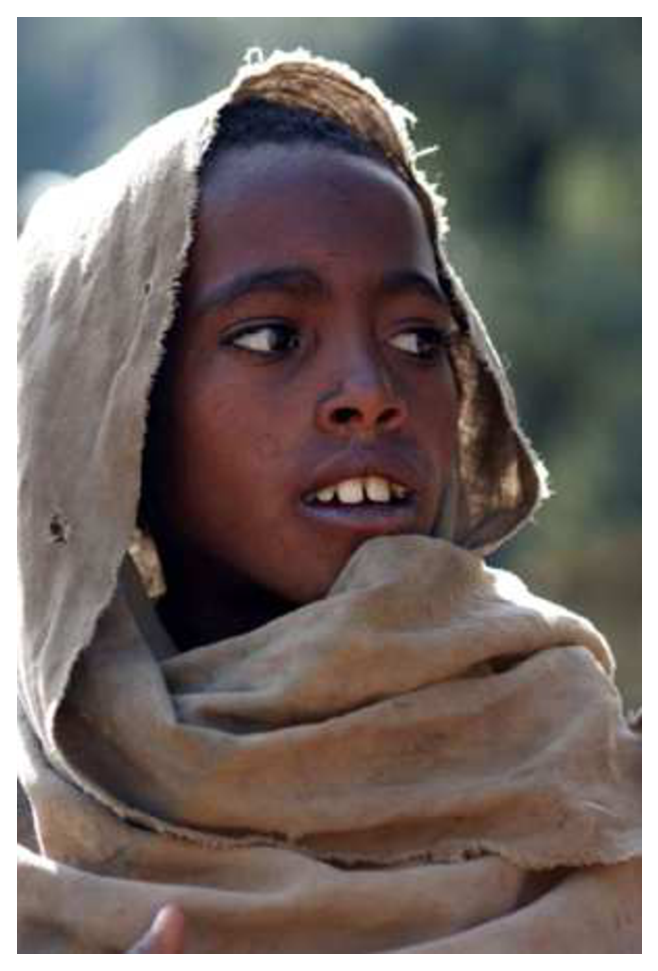
\includegraphics{etiopan.eps}\reflectbox{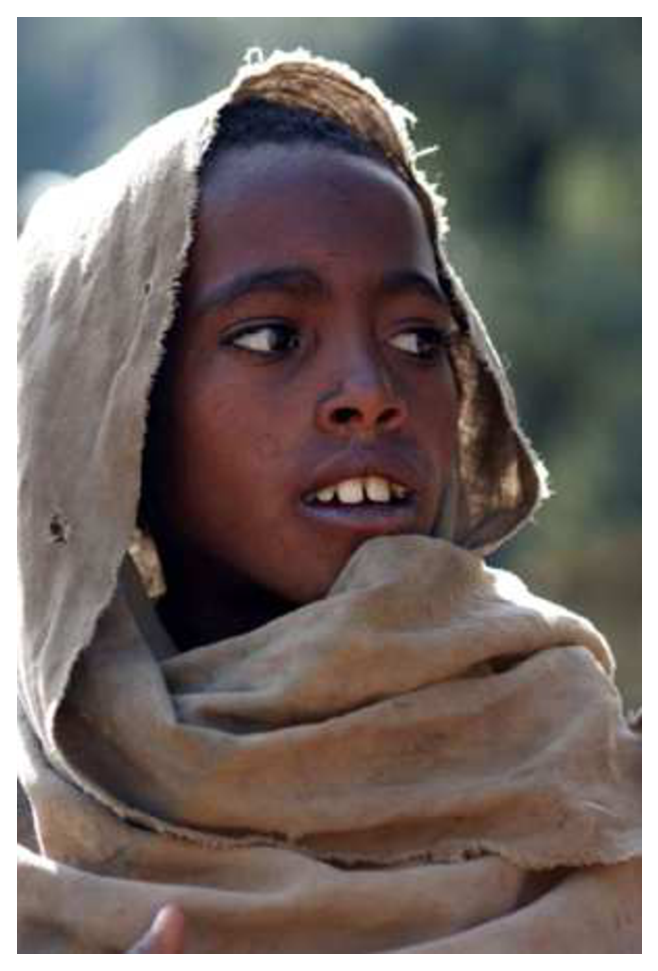
\includegraphics{etiopan.eps}}}}
\caption{Malý Etiopánek a jeho bratřícek} \label{obr.1}
\end{figure}
\newpage

Rozdíl mezi~vektorovým \dots

\begin{figure}[h]
\center{\scalebox{0.4}{
\includegraphics{oniisan.eps}}}
\caption{Vektorový obrázek} \label{obr.2}

\end{figure}

\dots a~bitmapovým obrázkem

\begin{figure}[h]
\center{\scalebox{0.6}{
\includegraphics{oniisan2.eps}}}
\caption{Bitmapový obrázek} \label{obr.3}

\end{figure}

\bigskip se projeví například při~zvětšení.

Odkazy (nejen ty) na~obrázky \ref{obr.1}, \ref{obr.2} a \ref{obr.3}, na  
tabulky \ref{tab.1} a~\ref{tab.2} a~také na~algoritmus \ref{algoritmus} jsou udělány pomocí 
křížových odkazů. Pak~je ovšem potřeba zdrojový soubor přeložit dvakrát.

Vektorové obrázky lze vytvořit i přímo v~\LaTeX{u}, například pomocí prostředí 
\texttt{ picture}.
\newpage
\begin{landscape}
\begin{figure}[ht]
\bigskip
\setlength{\unitlength}{0.5pt}
%%%\setlength{\unitlength}{4pt}
\begin{center}
\begin{picture}(1060, 530)(0,0) 
\put(0,0){\framebox(1060,530){}} %ramecek
\put(865,420){\circle{70}} %slunicko
\linethickness{5.3pt} 
\put(18,70){\line(1,0){1024}} %%%tlusta cara
%%%%%%%%cary tloustky 1pt%%%%%%%%%%%%%%%%%%
\linethickness{1pt} 
\put(138,70){\line(0,1){180}}
\put(192,76){\line(0,1){69}}
\put(138,250){\line(1,0){215}}
\put(192,145){\line(1,0){183}}
\put(354,223){\line(0,1){50}}
\put(354,273){\line(1,0){280}}
\put(232,223){\line(1,0){700}}
\put(232,194){\line(1,0){700}}
\put(232,194){\line(0,1){29}}
\put(932,194){\line(0,1){29}}
\put(634,223){\line(0,1){50}}
\put(634,238){\line(1,0){242}}
\put(876,223){\line(0,1){15}}
\put(393,181){\line(1,0){524}}
\put(393,136){\line(0,1){45}}
\put(930,70){\line(0,1){44}}
\put(436,115){\line(1,0){494}}
\put(918,115){\line(0,1){67}}
\put(232,194){\line(1,-1){48}}
\put(374,145){\line(2,{-1}){140}}
\end{picture}
\caption{Vektorový obrázek.}
\end{center}
\end{figure}
\end{landscape}
\end{document}
